\chapter{Fundamentos teóricos}\label{fundamentos}

Este capítulo descreve os principais elementos teóricos utilizados no
desenvolvimento desta pesquisa, é descrito neste capítulo um pouco da introdução histórica do problema de sequenciamento de tarefas.
\section{Introdução ao Sequenciamento de Tarefas}\label{sec:int_seq_tarefas}

A necessidade de técnicas de gestão das tarefas, tanto nos serviços quanto nas indústrias é cada vez mais crítica. Segundo \citeonline{ROLDAO}: O planejamento de operações é uma área em que se têm obtido mais progresso e cuja utilização traz mais vantagens ao gestor. 


O Sequenciamento de Tarefas, ou Scheduling, também chamado por alguns autores de Calendarização, pode ser definido como um processo de decisão para uma distribuição de recursos ao longo do tempo para realizar um conjunto de tarefas, sujeito a restrições (datas limites, duração e pendência das operações, tempos de movimentação e preparação, disponibilidade e partilha de recursos) e preferências – constrangimentos relaxáveis (relacionadas com datas limite, produtividade, frequência de troca de ferramentas e estabilidade da fábrica) \cite{LEPAPE}.

Nos problemas de Scheduling, de um modo geral, assume-se a necessidade de executar certo número de tarefas ou processos, cada um dos quais consiste numa dada sequência de operações, a executar pela ordem especificada na sequência, e usa certo número de maquinas. O processamento de uma operação requer o uso de uma maquina particular durante certo intervalo de tempo e cada maquina só pode processar uma operação de cada vez. É dada uma função que mede o custo de cada solução possível e pretende-se obter uma solução em que o custo seja mínimo.


O parâmetros para um problema de Scheduling de forma geral pode ser posto da seguinte forma:
\begin{itemize}
\item Existe um conjunto de $k$ operações, O = \{$O_{1}$, $O_{2}$, ... , $O_{k}$ \}
\item Existem um conjunto de $m$ maquinas, P = \{ $P_{1}$, $P_{2}$, ... , $P_{m}$\}
\item Pode haver um conjunto de $s$ Recursos adicionais, R = \{$R_{1}$, $R_{2}$,..., $R_{s}$\}

\end{itemize}


\section{Classificação das Máquinas}\label{sec:class_maq}
Segundo \citeonline{BLAZEWICZ} as maquinas podem ser classificadas de acordo com as funções que desempenham, sendo essa classificação feita do seguinte modo:

\begin{itemize}
\item {\bf Máquinas Paralelas}: Se todas as máquinas do conjunto P desempenham as mesmas funções. Elas podem ser distinguidas pelas suas velocidades de processamento. 

\item {\bf Máquinas Dedicadas}: Cada máquina do conjunto P é especializada na execução e uma operação específica.
\end{itemize}

\section{Variantes do Problema de Scheduling}\label{sec:Var_Prob}
Conforme explica \citeonline{CUNHA}, dependendo da classificação de um dado problema, existe também uma classificação dos Jobs Schedules, que é a forma como será tratado esse problema, ou seja, é a forma como os Jobs serão escalonados nas maquinas que os executam.

Existem basicamente três tipos de escalonamento: {\it Open-Shop}, {\it Flow-Shop} e {\it Job-Shop}. Uma vez identificado o tipo de problema, pode-se escolher uma destas estratégias para abordá-lo, abaixo segue uma rápida definição de cada um desses três tipos básicos de Scheduling.

\subsection{Open-Shop Scheduling}
Nesse tipo de problema as operações de cada um dos Jobs não possuem uma sequência para serem executadas. Dessa forma, as operações são totalmente independentes, não existindo restrições quanto à ordem de execução.
Através desse tipo de escalonamento, as tarefas precisam ser executadas por todas as máquinas e isso pode ocorrem em qualquer ordem, objetivando, também, minimizar o tempo total de execução que é chamado \textit{makespan} e o tempo total de fluxo denominado \textit{flowtime}.

\subsection{Flow-Shop Scheduling}
Neste tipo de problema existe uma ordem pré-estabelecida para execução das operações de cada um dos Job, ou seja, existe uma sequência de execução que deve ser respeitada. Neste caso, o processamento das tarefas ocorre em linha, ou seja, as tarefas passam por todas as máquinas que compõem o sistema, exatamente na mesma ordem, assim a {\it i}-ésima operação de cada uma das tarefas deverá ser sempre feita na máquina \textit{i}.

			Percebe-se que ao invés de se projetar o escalonamento de operações, faz-se o planejamento das tarefas em relação ao uso das máquinas.

\subsection{Job-Shop Scheduling}
O Job-Shop Scheduling caracteriza-se por diferenciar as operações de cada um dos Jobs, direcionando sua execução para máquinas específicas, o que restringe a execução de uma dada operação a uma só máquina, e pode existir um caso de ter mais de uma máquina do mesmo tipo \cite{PINEDO}. Esse tipo de escalonamento permite que se estabeleçam diversas escalas, vez que pode haver flexibilidade quanto à ordem de processamento das operações, bem como, quanto à ordem de utilização das máquinas, que deve objetivar o tempo mínimo de ociosidade e o mínimo tempo total da execução (makespan). Essa medida de qualidade, conhecida como \textit{makespan}, não é a única existente, porém é o critério mais simples e mais utizado.  O objetivo implica em buscar arranjos de operações cuja ordem de execução em cada maquina leve o menor tempo possível, ou seja, a melhor solução para o problema.

O Job Shop Scheduling é composto por um conjunto de Jobs (J = $\{j_1, j_2, ...,j_p\}$), onde cada job é composto por um conjunto de operações ($ j_i=\{ o_{i1}, o_{i2}, ..., o_{ip} \} $) e cada operação tem seu tempo de processamento, todos os tempos de processamento de cada operação formam um conjunto de tempos de processamento ($t_i=\{t_{i1}, t_{i2}, ...,t_{ip}\} $), onde cada tempo pode ser identificado em relação as respectivas operações, assim, $t_{ip}$ é o tempo de processamento da \textit{p}-ésima operação do \textit{i}-ésimo job. Em termos de complexidade de processamento o \textit{Job Shop} corresponde ao problema de \textit{Scheduling} mais genérico e mais complexo.

\section{Notação}

\begin{description}

\item [Job-Shop ($J_{m})$]: O $J_m$ representa um Job Shop com {\it m} máquinas, onde cada job tem sua rota predeterminada a seguir.

\item [Tempo de Processamento ($P_{ij}$)]: O tempo de processamento $P_{ij}$ representra o tempo de processamento do Job {\it j} na máquina {\it i}. O subscrito {\it i} pode ser omitido quando o tempo de processamento do Job {\it j} não depende da máquina ou se ele é processado por apenas uma máquina.

\item [Data de início ($r_j$)]: A data de ińicio do Job {\it j}, representado pela letra $r_j$, é o tempo (data) que o Job chega no sistema, indica o tempo que o job {\it j} pode começar a ser processado

\item [Data de vencimento ($d_j$)]: A data de vencimento $d_j$ do Job {\it j} representa a data de finalização do processamento do Job {\it j}, é o quem é chamado de tempo de pronto.

\item [Makespan ($C_{max}$)]: O Makespan pode ser chamado de tempo de fabricação, é tempo final de processamento de todos os jobs, e é definido como max ($C_1$, … , $C_n$).
\end{description}

Para o caso de Makespan mínimo ( $J_m \parallel C_{max}$ ) a seguinte programação matemática pode ser utilizada.

$\\Minimize\ C_{max}\\ \\
sujeito\ a$
\begin{eqnarray*}
        y_{kj}-y_{ij}\geq p_{ij} \qquad \qquad \quad \forall (i,j) \rightarrow (k,j) \in A  \quad (1)\\
        C_{max} – y_{ij}\geq p_{ij} \qquad \qquad \qquad \qquad \quad \forall (i,j) \in N \quad (2)\\
        y_{ij}-y_{i1}\geq p_{i1}\quad ou \quad y_{i1}-y_{ij}\geq p_{ij} \qquad \qquad\forall(i,1) e (i,j) = 1, ..., m \quad (3) \\
         y_{ij}\geq 0 \qquad \qquad \quad \qquad \qquad \qquad \qquad \qquad (4)
\end{eqnarray*}

onde,
\begin{itemize}

\item $y_{ij}$ é o tempo inical de processamento do Job {\it j} na máquina {\it i};
\item $p_{ij}$ é a duração do job {\it j} na máquina {\it i}
\item $N$ é o conjunto de todas as operações $(i,j)$
\item $A$ é conjunto de todas as restrições de rotas $(i,j) \rightarrow (k,j)$
\item $m$ é o número total de máquinas

\end{itemize}

\section{Representação do Problema}\label{sec:rep_prob}
Um \textit{Job-Shop Scheduling} é a representação de uma programação dos Jobs, compostos por operações interdependentes, onde cada Job deve ser processado por uma máquina diferente. A solução para o problema de Job-Shop Scheduling pode ser representada de duas formas: Gráfico de Gant e Grafos Disjuntivos.

\subsection{Gráfico de Gantt}
Desenvolvido em 1917 pelo engenheiro mecânico Henry Gantt, o Gráfico de Gantt representado na figura \ref{graf_gantt} é usado para representar uma solução para o problema de Job Shop Scheduling, ele exibe um possível seqüenciamento de execução das operações por parte das maquinas.

\begin{figure}[H]
\centering
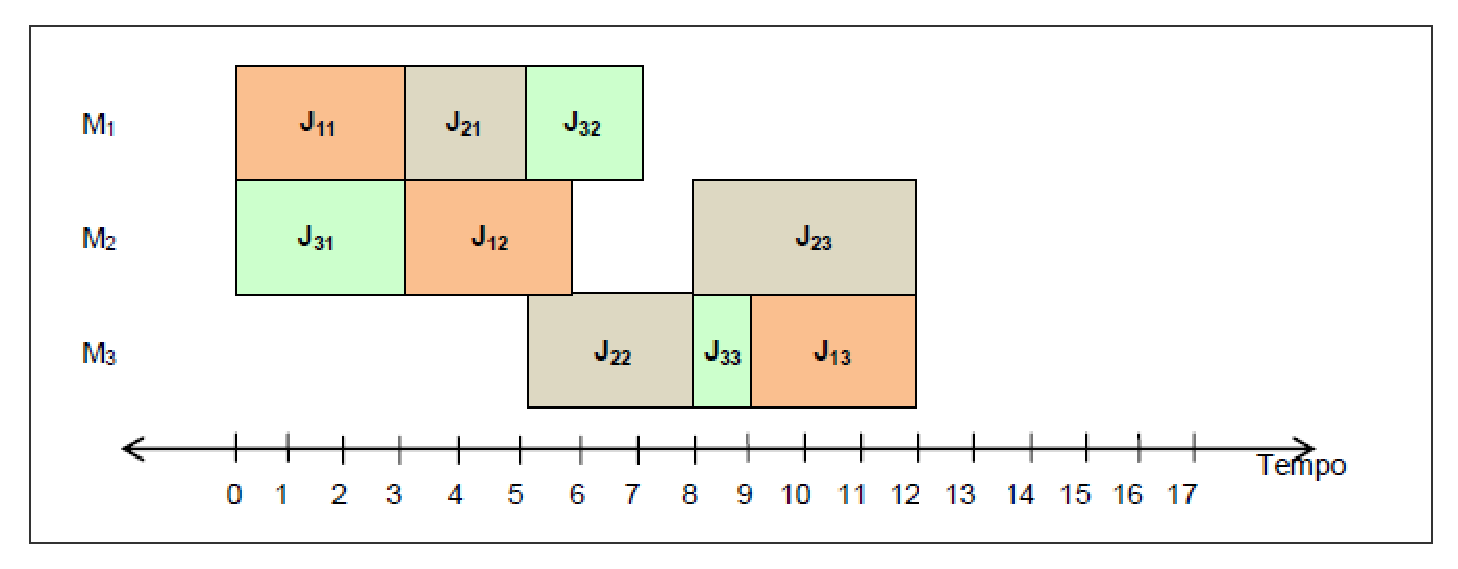
\includegraphics[scale = 0.6]{graficos/graf_gantt.eps}
\caption{Representação pelo Grafico de Gantt}
\label{graf_gantt}
\end{figure}

Nesse gráfico o eixo vertical representa as maquinas, o eixo horizontal representa a linha do tempo, e os retângulos representam as operações que compõem os Jobs, eles são encaixados no gráfico de modo que o seu tempo de execução fique marcado na linha do tempo. Os Jobs são identificados facilmente pela cor do retângulo, por exemplo, o Job 1 está representado pela cor laranja, onde $J_{11}$ representa a operação 1 do Job 1, o $J_{12}$ representa a operação 2 do Job 1 e o $J_{13}$ representa a operação 3 do Job 1. Com base na representação da solução da figura 1 o \textit{makespan}, ou seja, o tempo total de conclusão das operações é igual a 12 unidades de tempo.

\subsection{Grafos Disjuntivos}
Grafos Disjuntivos podem ser usados tanto para modelar um problema de \textit{Scheduling}, quanto para representar sua solução. A idéia principal dele consiste em mostrar a solução do problema destacando o uso das máquinas, e respeitando a precedência de operação dos Jobs. 

\subsubsection{Representação do Problema}
Um grafo parcialmente orientado, constituído por outros grafos pode ser usado como uma representação que reúne as características mais relevantes para o projeto de escalonamento de um problema de \textit{Job Shop Scheduling}. Uma representação do problema de \textit{Job Shop Scheduling} pode ser visualizada pelo Grafo Disjuntivo ilustrado na figura \ref{grafo_disjunt} 

\begin{figure}[H]
\centering
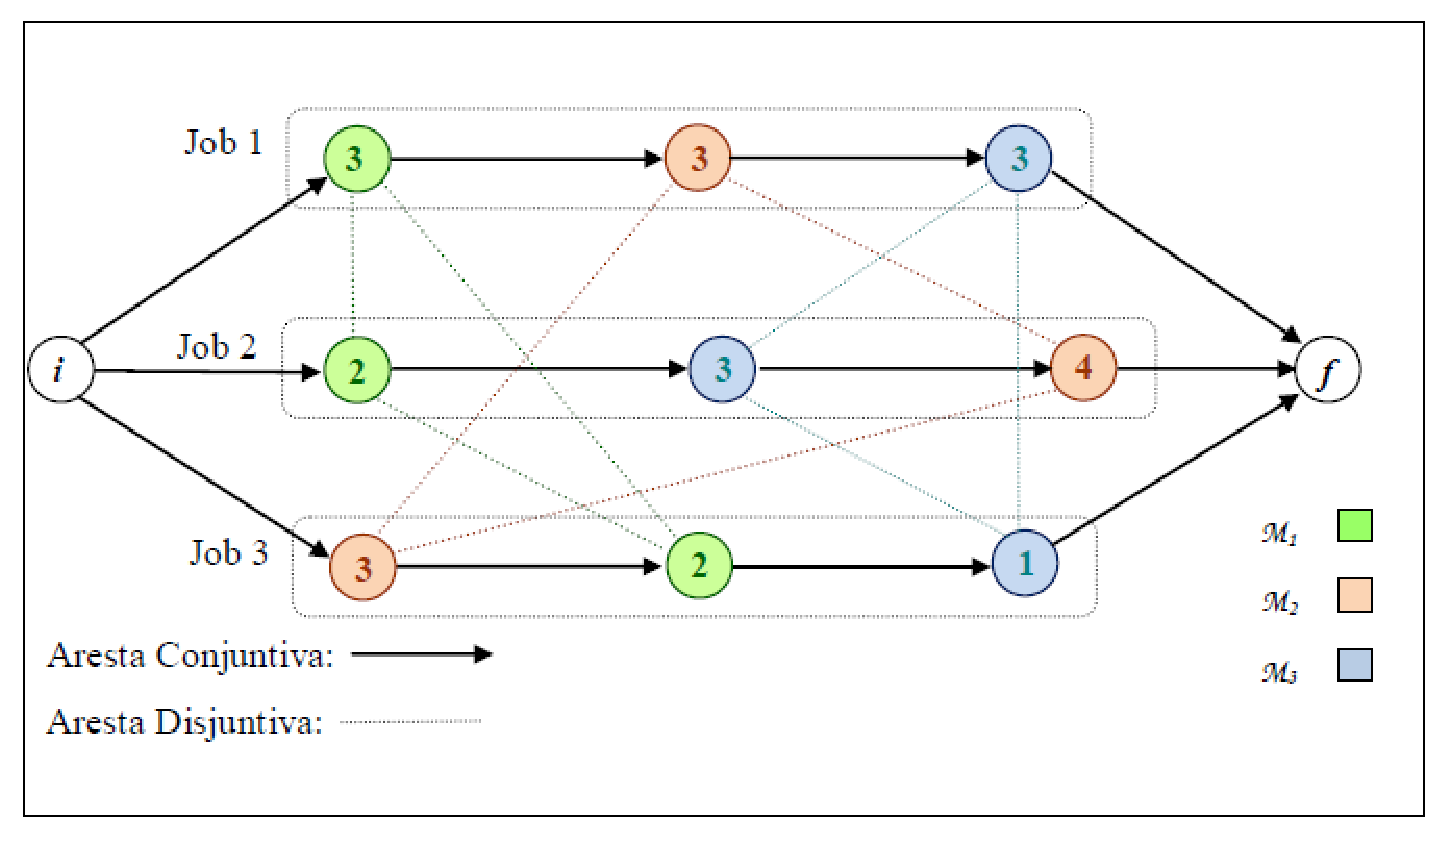
\includegraphics[scale = 0.6]{graficos/grafo_disjuntivo.eps}
\caption{Representação do problema usando grafo disjuntivo}
\label{grafo_disjunt}
\end{figure}

As operações de um mesmo Job estão interligadas por uma relação de dependência de prioridade de execução. Esta ligação é representada por arestas horizontais orientadas em um único sentido, as quais formam o grafo conjuntivo e elas não podem sofrer modificações de sentido. Cada operação deve ser executada por uma máquina diferente, as cores de cada job indica em qual máquina ele é executado, a interconexão não orientada forma o grafo disjuntivo, e relaciona os jobs que são executados pela mesma máquina, o número representado em cada operação na figura acima indica o tempo de processamento da operação.

\subsubsection{Representação da Solução}
Uma possível solução para o problema de Job Shop Scheduling pode ser representada por uma simples orientação do grafo disjuntivo, como mostra a Figura \ref{grafo_disj_orient}, lembrando que, somente as arestas disjuntivas podem sofrer modificações, pois elas indicam o escalonameto da máquina, e as arestas conjuntivas representam a restrição de precedência de operações.
	
Realizar um escalonamento das operações constituintes significa buscar uma solução para o problema, esse escalonamento das operações possui uma certa flexibilidade, pode ser alcançar diversas possibilidades de arranjo das operações, mas o grafo disjuntivo deve ser manter acíclico, pois uma operação só pode ser executada por uma máquina apenas uma vez.

\begin{figure}[H]
 \centering
 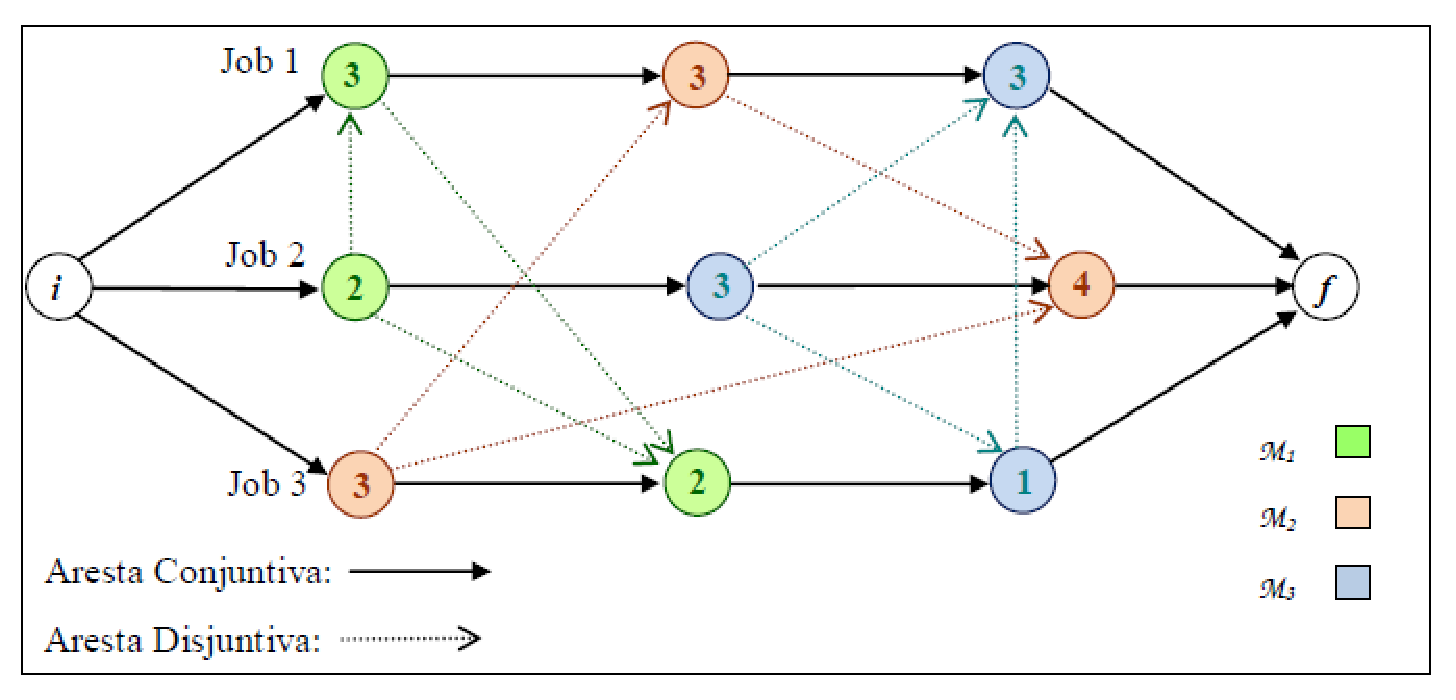
\includegraphics[scale = 0.6]{graficos/grafo_disjuntivo_orientado.eps}
 \caption{Representação da solução usando grafo disjuntivo orientado}
 \label{grafo_disj_orient}
\end{figure}

A solução encontrada através do escalonamento das operações no grafo disjuntivo necessita ser avaliada e comparada com outras soluções, uma forma de avaliação é analisar o tempo do caminho crítico, isto é, analisar o tempo de execução das operações mais demoradas \textcolor{red}{assim a solução encontrada deve ser menor que a análise do caminho crítico}.

\section{Métodos de Solução} \label{sec:met_sol}
O problema de \textit{Job Shop Scheduling} é classificado como NP-difícil, ou seja, é um problema para o qual não existem algoritmos que o resolva em tempo polinomial. Trata-se de um “Problema de Otimização Combinatória” \cite{SOUZA}.
Os algoritmos de solução podem ser classificados em duas classes:  Modelos matemáticos e Modelos heurísticos.

\begin{itemize}
\item \textbf{Modelos Matemáticos}: Trata-se de modelos de programação inteira mista, resolvidos pelos métodos branch and bound ou branch and cut.  Modelos Matemáticos enfatizam a obtenção de resultados ótimos em função de algum parâmetro de desempenho. Este pode ser, por exemplo, a minimização dos tempos de produção ou a maximização do uso dos recursos. Dependendo da complexidade do problema tratado, o calculo da solução ótima pode ser computacionalmente inviável.

\item \textbf{Modelos Heurísticos}: Trata-se de modelos baseados em regras pratica de escalonamento que enfatiza a obtenção de “boas” soluções, próxima da solução ótima. Os modelos heurísticos são caracterizados por obter uma solução aproximada em tempos de computação viáveis. 
\end{itemize}

\section{O problema de Sequenciamento de Tarefas e suas Aplicações}
A programação de tarefas constitui-se num alvo de pesquisa a ser buscado por fábricas de diversas designações, as quais disponham de máquinas destinadas a papéis específicos com o fim de produzir, comumente, mais de um tipo de produto e, às vezes, utilizando uma mesma máquina em alguma etapa do processo; com o objetivo de minimizar o tempo ocioso e maximizar a produtividade.

Embora o nome seqüenciamento de tarefas parece sugerir que o problema seja aplicado no ramo de produção industrial, ele ocorre em variados contextos, pode ser um ambiente de aplicação do problema, por exemplo, a distribuição de médicos e enfermeiros de um hospital, turmas e professores em uma sala de aula, navios em um porto, cidades e caxeiros viajantes, etc. \cite{REIS}



